\section{Contiki-ng}
\label{contikiNG}

Contiki es un sistema operativo enfocado a sensores de baja capacidad. Este sistema operativo fue desarrollado por Adam Dunkels con la ayuda de  Bjorn Gronvall y Thiemo Voigt en el año 2002. Desde entonces hasta los últimos años, el proyecto Contiki  ha involucrado tanto a empresas como a cientos de colaboradores en su repositorio de GitHub\footnote{\url{https://github.com/contiki-os/contiki}}.  Contiki estaba diseñado con el propósito de ofrecer a los nodos de las redes \gls{wsn} un sistema operativo ligero con capacidad de carga y descarga de servicios únicos de forma dinámica \cite{1367266}. \\
\par
El Kernel de Contiki está orientado a eventos, y soporta tareas multi-hilo con requisa. Contiki está escrito en el lenguaje C y ha sido portado a numerosas de arquitecturas de microcontroladores, como el MSP430 de Texas Instruments y derivados. \\
\par

En un sistema que ejecute el sistema operativo de Contiki, éste estará dividido en dos partes claramente diferenciadas según se puede ver en la figura \ref{fig:contikiParts}, el \textit{core} y los programas o servicios cargados. El particionado se lleva a cabo en el momento de la compilación y es independiente de cada target en el que se vaya a desplegar el sistema. El \textit{core} consiste en el propio Kernel, un conjunto de servicios de base (\textit{timers}, \textit{handlers}) , librerías, drivers y el \textit{stack} de comunicación. Los programas o servicios cargados se mapearán en memoria por el propio cargador que tiene el Kernel en tiempo de ejecución.\\
\par


% Foto 
\begin{figure}[ht]
    \centering
    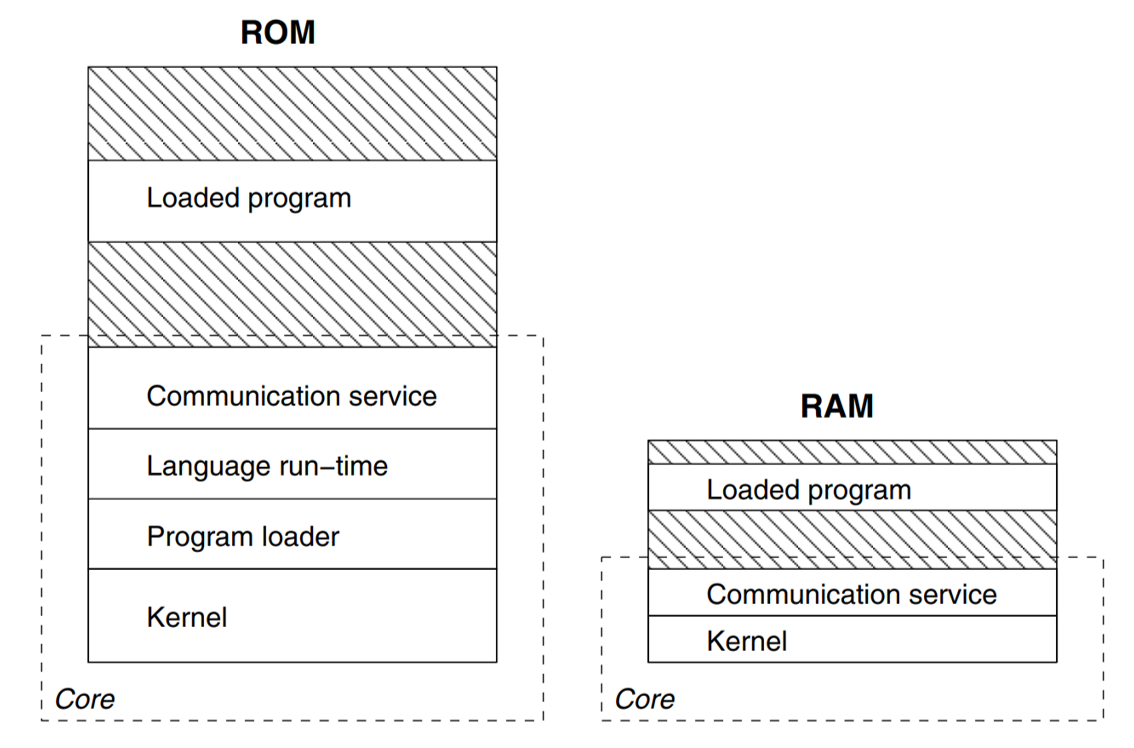
\includegraphics[width=9.5cm]{archivos/img/teoria/contiki.png}
    \caption{Particionado en un sistema con Contiki OS \cite{1367266}}
    \label{fig:contikiParts}
\end{figure}

En los últimos años apareció un nuevo proyecto, \textbf{Contiki-ng} \footnote{\url{https://github.com/contiki-ng/contiki-ng}}, el cual es fork de Contiki OS. Este nuevo proyecto desbancaría a su predecesor bajo el eslogan de ``\textit{Contiki-NG: The OS for Next Generation IoT Devices}". Actualmente toda la comunidad de Contiki está enfocada en este nuevo proyecto, el cual proporciona un \textit{stack} de comunicación más cercano a las RFCs, soporte a protocolos como IPv6/6LoWPAN y 6TiSCH, y por lo que se está haciendo más popular, dar soporte a microcontroladores con la arquitectura ARM \cite{kurniawan2018practical}.
\vspace{0.5cm}


\subsection{Simulador Cooja}

El flujo de trabajo con Contiki o Contiki-ng, dependerá si se va a trabajar sobre hardware real o si se va a simular los programas desarrollados. Cuando se trabaja sobre hardware real, el flujo de trabajo consistirá en la compilación del sistema operativo y de los programas desarrollados con el target donde se vaya a trabajar, generando así un binario el cual se podrá instanciar en el disco del hardware. \\

\par
Si por el contrario se va a simular, se hará uso del simulador llamado Cooja\footnote{\url{https://github.com/contiki-ng/cooja/tree/master}}. Cooja es una simulador escrito en Java que permite simular una serie de motas \gls{iot}. Por tanto, a la hora de simular se podrá ver el comportamiento del programa desarrollado en distintas plataformas. \\
\par

Todo el proceso de compilación del \textit{core} de Contiki y programas desarrollados está integrado en el propio simulador, permitiendo al usuario compilar sus programas hacia distintos tipos de motas. Cada simulación se podrá almacenar en un fichero con la extensión \texttt{*.csc}, los cuales almacenarán todos los datos de la simulación, \textit{seed}, posiciones y tipos de motas en una estructura XML. \\
\par


% % Foto 
% \begin{figure}[ht]
%     \centering
%     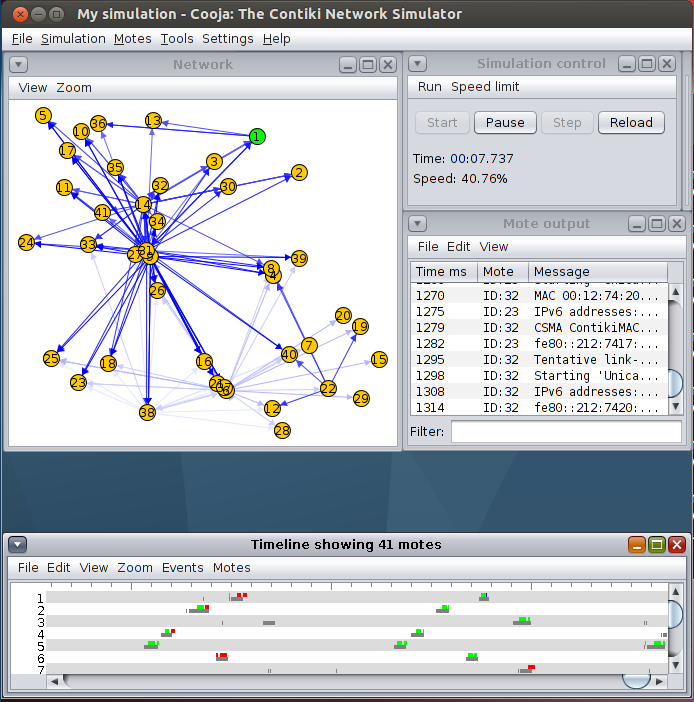
\includegraphics[width=13.5cm]{archivos/img/teoria/cooja.png}
%     \caption{GUI Simulador Cooja \cite{cooja}}
%     \label{fig:cooja}
% \end{figure}